% !TeX root = ../presentation.tex

\section{Data Spaces}

\begin{frame}{Inter-Organisational Information Systems (IOIS) \footnotesize\cite{mollerIndustrialDataEcosystems2024}}
    \begin{columns}
        \begin{column}{0.6\textwidth}
            \begin{itemize}
                \item \alert{bilaterale} Beziehungen, bspw. Lieferketten
                \item tiefe Integration, automatisiertes Data Sharing
                \item zweckgebunden, bspw. Koordinierung und Optimierung von Lieferketten
                % Mittel zum Zweck
                
                \item<2-> mangelndes Vertrauen, streng formalisierte Nutzungsrichtlinien
                \item<2-> keine Daten teilen? $\to$ Ineffizienz $\to$ Verlust
                \item<2-> Herausforderungen bei Skalierung % Datenaustausch, Kontrolle
            \end{itemize}
        \end{column}
        
        \begin{column}{0.4\textwidth}
            \begin{figure}
                
\includegraphics[height=0.5\textheight]{./assets/iois_architecture.drawio.pdf}
                \caption{IOIS Architektur}
            \end{figure}
        \end{column}
    \end{columns}
\end{frame}


\begin{frame}{Data Intermediaries \footnotesize\cite{mollerIndustrialDataEcosystems2024}}
    \begin{columns}
        \begin{column}{0.6\textwidth}
            \begin{itemize}
                % dynamisch, geteilter Zweck
                \item Gleichgewicht zwischen erhaltenem und gegebenem Aufwand
                \item Daten als strategische Ressource % statt Mittel zum Zweck
                % ermöglichen neue Geschäfte und Optimierung von Prozessen
                
                \item<2-> Interaktion und Kooperation \alert{multilateraler} Akteure
                \item<2-> Data User, Data Provider, Data Intermediary
                
                \item<3-> offener, dynamischer Datenaustausch
                \item<3-> Netzwerkeffekte, Förderung von Innovation
            \end{itemize}
        \end{column}
        
        \begin{column}{0.4\textwidth}
            \begin{figure}
                \centering
                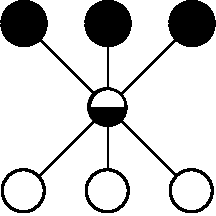
\includegraphics[height=0.5\textheight]{./assets/industrial_de_architecture.drawio.pdf}
                \caption{Data Intermediary}
            \end{figure}
        \end{column}
    \end{columns}
\end{frame}


\begin{frame}{Data Spaces \footnotesize\cite{mollerIndustrialDataEcosystems2024}}
    \begin{columns}
        \begin{column}{0.6\textwidth}
            \begin{itemize}
                \item Vereinen von IOIS und Data Intermediaries
                \item dezentrale Speicherung von Daten bei Provider
                
                \item<0|handout:0> Datenintegration auf semantische Ebene
                \begin{itemize}
                    \item[$\to$]<0|handout:0> kein einheitliches Daten"=Schema notwendig
                \end{itemize}
                \item<0|handout:0> bilateraler Datenaustausch
                \item<0|handout:0> Vermittlung zwischen Data User und Provider
                \item<0|handout:0> technische Garantie von Datensouveränität
                \item<0|handout:0> geteilter Raum für vertrauenswürdiges Data Sharing $\to$ Optimierung, Innovation
            \end{itemize}
        \end{column}
        
        \begin{column}{0.4\textwidth}
            \begin{figure}
                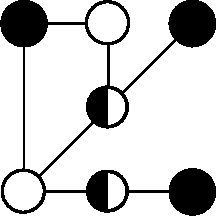
\includegraphics[height=0.5\textheight]{./assets/data_space_architecture.drawio.pdf}
                \caption{Data Space Architektur}
            \end{figure}
        \end{column}
    \end{columns}
\end{frame}


\begin{frame}[c]{Einschub: Zentrale vs. Dezentrale Datenspeicherung}
    \vspace{1.5em}

    \begin{figure}
        \centering
        \begin{subfigure}{0.4\textwidth}
            \centering
            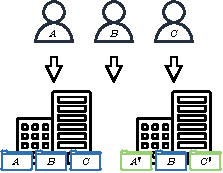
\includegraphics[height=5cm]{./assets/central.drawio.pdf}
        \end{subfigure}
        % Duplikat --> Inkonsistenz
        %
        \hspace{2cm}
        %
        \only<2->{
            \begin{subfigure}{0.4\textwidth}
                \centering
                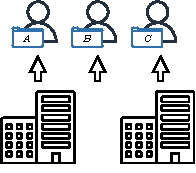
\includegraphics[height=5cm]{./assets/decentral.drawio.pdf}
            \end{subfigure}
        }
        % Daten bei Nutzenden / Data Provider ---> Konsistenz
        % Kontrolle über Zugang, nur wenn notwendig

        \caption{zentralisierte vs. dezentralisierte Datenspeicherung}
    \end{figure}
\end{frame}


\begin{frame}{Data Spaces \footnotesize\cite{mollerIndustrialDataEcosystems2024}}
    \begin{columns}
        \begin{column}{0.6\textwidth}
            \begin{itemize}
                \item Vereinen von IOIS und Data Intermediaries
                \item dezentrale Speicherung von Daten bei Provider
                
                \item<2-> Datenintegration auf semantische Ebene
                \begin{itemize}
                    \item[$\to$]<2-> kein einheitliches Daten"=Schema notwendig
                \end{itemize}
                
                \item<3-> bilateraler Datenaustausch % vgl. IOIS
                \item<3-> Vermittlung zwischen Data User und Provider % vgl. Data Intermediary
                % Adapter --> reines Mapping + Weitergeben
                % Mediator --> Kontroll-Möglichkeiten

                % prinzipiell überhaupt eine Chance, dass ich an benötigte Daten komme
                % --> Daten-Lieferketten, muss zu best. Domäne kommen
                
                \item<4-> technische Garantie von Datensouveränität
                % -> Überwindung betriebl. Barrieren
                % Kontrolle über Zugriff und Verwendung bei Provider
                \item<4-> geteilter Raum für vertrauenswürdiges Data Sharing $\to$ Optimierung, Innovation
                % flexible betriebliche Strukturen
                % Zugang nur für bestimmte Akteure --> *Trusted Pool*
                % sicheres, vertrauenswürdiges Data Sharing
            \end{itemize}
        \end{column}
        
        \begin{column}{0.4\textwidth}
            \begin{figure}
                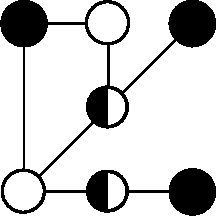
\includegraphics[height=0.5\textheight]{./assets/data_space_architecture.drawio.pdf}
                \caption{Data Space Architektur}
            \end{figure}
        \end{column}
    \end{columns}
\end{frame}


\begin{frame}{Data Ecosystems \footnotesize\cite{mollerIndustrialDataEcosystems2024}}
    \begin{columns}
        \begin{column}{0.6\textwidth}
            \begin{itemize}
                % Kapselung möglich, DS ist nur weiterer Data Provider
                \item Kapselung $\to$ Data Space als Data Provider
                % merkt man nicht, wenn DS größer wird
                
                \item[$\Rightarrow$] \emph{globaler} Data Space?
                \begin{itemize}
                    \item<2-> Domänen-spezifisch, starke Kopplungen
                    % Datenstrukturen für spez. genau für diesen Teilbereich, aber trotzdem verknüpft
                    % jede Domäne hat noch weitere Daten, interessiert andere Seite nicht
                \end{itemize}

                % daher
                \item<3-> eigene Data Spaces für Domäne
                    % erfüllen genau diesen gemeinsamen Zweck
                \item<3-> über Data Space hinweg: lose Kopplung
                % bspw. komplette Medizindaten beim Arzt vs. nur relevante Daten für Studie
                % Details sind uninteressant

                \item[$\Rightarrow$]<4-> Verschachtelung / Überlappung von Data Spaces
                \item[$\Rightarrow$]<4-> \alert{\emph{Data Ecosystem}}
                    % um einen oder mehrere föderierte Data Spaces
                    % technische Integration über Schnittstellen
                    % Datensouveränität & Verhinderung großer Daten-Silos: verschachtelt && überlappend

                    % Bild: Punkte können Data Prov. oder DS sein --> Kapselung, Verschachtelung
                    % orangene Linien: Verbindung von Data Spaces, lose Kopplung
                    % oben rechts: kein Teilnehmer aus DS von unten, aber trotzdem Zugriff auf rel. Daten
                

                % prinzipiell überhaupt eine Chance, dass ich an benötigte Daten komme
                % --> Daten-Lieferketten, muss zu best. Domäne kommen
                % brauche Kontrollen --> DS Connectors
                \item<5-> Integration über \emph{Data Space Connector}
                % vgl. Adapter (nur Weitergabe) oder Mediator (inkl. Kontrollmechanismen)
                % Kontrolle notwendig --> DS Connectors
                % bspw. Weitergabe von med. Daten an Forschungsinstitut
                %   muss anonymisiert erfolgen, nur best. Daten dürfen weitergegeben werden
                \item<5-> Governance"=Maßnahmen je Abstraktionsebene
                % Erfüllung rechtlicher Rahmenbedingungen
                % Ebene von DE, DS, Pod oder Ressourcen
                \item<5-> Erreichen gemeinsamer Ziele
            \end{itemize}
        \end{column}

        \begin{column}{0.4\textwidth}
            \only<4->{
                \begin{figure}
                    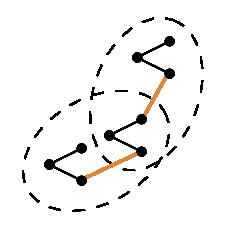
\includegraphics[height=5cm]{./assets/data_ecosystem_architecture.drawio.pdf}
                    \vspace{-1em}
                    \caption{Data Ecosystem}
                \end{figure}
            }
        \end{column}
    \end{columns}

    % Data Spaces erfüllen am meisten Kriterien
    % Wie kann das funktionieren? --> Solid
\end{frame}
